\documentclass[a4paper,twoside]{article}

% \usepackage{cite}
% \usepackage[numbers]{natbib}
\usepackage{amsmath,amssymb,amsfonts}
\usepackage{algorithmic}
\usepackage{graphicx}
\usepackage{textcomp}
\usepackage{xcolor}

% Table stuff
\usepackage{booktabs}
\usepackage{multirow}
\usepackage{longtable}

% Figure stuff
\usepackage{tikz}
\usepackage{fancyvrb}

% SCITEPRESS packages
% \usepackage{epsfig}
% \usepackage{epstopdf}
\usepackage{subcaption}
\usepackage{calc}
\usepackage{amssymb}
\usepackage{amstext}
\usepackage{amsmath}
\usepackage{amsthm}
\usepackage{multicol}
\usepackage{pslatex}
\usepackage{apalike}
\usepackage[bottom]{footmisc}
\usepackage{SCITEPRESS}

% \epstopdfsetup{outdir=./}
% \epstopdfsetup{outdir = ./}

% Bibliography
\bibliographystyle{apalike}
% \addbibresource{references.bib}

\begin{document}

\title{A Framework for Assessing Decompiler Inference Accuracy of Source-Level Program Constructs}

\author{\authorname{Jace Kline\sup{1}\orcidAuthor{0000-0003-4442-9776}, Prasad Kulkarni\sup{1}\orcidAuthor{0000-0000-0000-0000}}
\affiliation{\sup{1}Department of Electical Engineering and Computer Science, University of Kansas, Lawrence, Kansas, United States}
\email{\{jace\_kline, prasadk\}@ku.edu}
}

\keywords{Decompilers, Security}

\abstract{Decompilation is the process of reverse engineering a binary program into an equivalent source code representation with the objective to recover high-level program constructs such as functions, variables, data types, and control flow mechanisms. Decompilation is applicable in many contexts, particularly for security analysts attempting to decipher the construction and behavior of malware samples. However, due to the loss of information during compilation, this process is naturally speculative and thus is prone to inaccuracy. This inherent speculation motivates the idea of an evaluation framework for decompilers. In this work, we present a novel framework to quantitatively evaluate the inference accuracy of decompilers, regarding functions, variables, and data types. Within our framework, we develop a domain-specific language (DSL) for representing such program information from any "ground truth" or decompiler source. Using our DSL, we implement a strategy for comparing ground truth and decompiler representations of the same program. Subsequently, we extract and present insightful metrics illustrating the accuracy of decompiler inference regarding functions, variables, and data types, over a given set of benchmark programs. We leverage our framework to assess the correctness of the Ghidra decompiler when compared to ground truth information scraped from DWARF debugging information. We perform this assessment over a subset of the GNU Core Utilities (Coreutils) programs and discuss our findings.}

\onecolumn \maketitle \normalsize \setcounter{footnote}{0} \vfill

\section{\uppercase{Introduction}} \label{sec:introduction}

\subsection{Context}

In an increasingly digital world, cybersecurity has emerged as a crucial consideration for individuals, companies, and governments trying to protect their information, financial assets, and intellectual property. Of the many digital threats, various forms of malware continue to pervade the digital landscape. \emph{Decompilation}, the translation from binary code into an approximate source-level representation, is a key strategy in attempting to understand the construction and behavior of malware samples. A \emph{decompiler} is a program that performs decompilation. The decompilation process is inherently speculative and error-prone since high-level information such as function boundaries, variables, data types, and control flow mechanisms are lost during program compilation. 

Due to this imprecise nature of decompilation, a generalized and extensible quantitative evaluation framework for decompilers is critical. Existing work \cite{bib:how-far-weve-come} proposes an evaluation technique to determine whether recompiled decompiled programs are consistent in behavior to their original binaries. Another work \cite{bib:metrics-effectiveness-decompilers} proposes a set of metrics for assessing the clarity of decompiled Java programs with respect to program size, conditional complexity, identifier complexity, number of local variables, and expression complexity. These works, although insightful for assessing decompiler quality, do not measure the recovery accuracy of high-level program constructs such as functions, variables, and data types. The recovery and inference of the these high-level constructs, in conjunction with clarity and behavioral correctness, is important for analysts to gain an understanding of decompiled binary programs.

Targeting the current gap in the literature, this paper presents a novel framework for quantifying and assessing the accuracy of decompiler tools with respect to high-level program constructs, including functions, variables, and data types. To prove our concept, we apply our framework to the Ghidra \cite{bib:ghidra} decompiler and discuss our findings. The primary objectives achieved by this work are as follows:

\begin{enumerate}
    \item We define a domain-specific language (DSL), written in Python, for expressing high-level program information including functions, variables, and data types. This serves as a medium whereby we can translate program information extracted from a decompiler or a ground-truth source.
    \item We extend our DSL to compare program information representations from different sources. The primary use case is to compare ground-truth program information to decompiler-inferred program information.
    \item Leveraging the comparison logic in (2), we define a set of quantitative metrics to measure the accuracy of function, variable, and data type inference.
    \item We develop a translation module in Python that uses DWARF debugging information from a binary program to generate a ground-truth program information representation in our DSL.
    \item We utilize the Ghidra Python API to implement a translation module. This module takes Ghidra decompilation of a binary program as input and outputs a program information representation in our DSL.
    \item Using our developed language, metrics, and translation modules, we quantitatively assess the accuracy of the Ghidra decompiler when compared to ground truth program information obtained from DWARF debugging information. We peform this analysis using the set of GNU Coreutils programs as benchmarks. We present the evaluation results and discuss additional findings and takeaways.
\end{enumerate}

The remainder of this paper is outlined as follows: In Section \ref{sec:background-related-work}, we discuss related research and background concepts useful for the understanding of this work. Next, in Section \ref{sec:methodology}, we detail our methodology for developing our evaluation framework. In Section \ref{sec:evaluation}, we present and discuss the results of applying our evaluation framework to the Ghidra decompiler. We conclude in Section \ref{sec:conclusion} with a summary of our results, implications of our work, limitations, and future research directions.

\section{\uppercase{Background and Related Work}} \label{sec:background-related-work}

\subsection{DWARF Debugging Standard}

\emph{DWARF} \cite{bib:dwarf} is a debugging file format used by many compilers and debuggers to support source-level debugging for compiled binary programs. When specified flags (usually '-g') are present at compilation, DWARF-supporting compilers such as GCC and Clang will augment the outputted binary program or object file with DWARF debugging information. A resulting binary executable can then be loaded into a DWARF-supporting debugger such as GDB to debug the target binary program with references to line numbers, functions, variables, and types in the source-level program. The DWARF standard is source language agnostic, but generally supports equivalent representations for constructs present in common procedural languages such as C, C++, and Fortran. In addition, DWARF is decoupled from any architecture or operating system. The generalizability of DWARF debugging information makes it a prime candidate for extracting "ground truth" information about a particular binary program, regardless of the specifics of the source language, architecture, or operating system. DWARF is leveraged in this work to obtain ground truth information about target binary programs.

\subsection{Ghidra Reverse Engineering Framework}

\emph{Ghidra} \cite{bib:ghidra}, created and maintained by the National Security Agency (NSA) Research Directorate, is an extensible software reverse engineering framework that features a disassembler, decompiler, and an integrated scripting environment in both Python and Java. We use the Ghidra decompiler in this work to demonstrate our decompiler evaluation framework.

\subsection{Related Work}

In a 2020 paper \cite{bib:how-far-weve-come}, the authors present an approach to determine the correctness of decompilers outputting C source code. They aim to find decompilation errors, recompilation errors, and behavior discrepancies exhibited by decompilers. To evaluate behavioral correctness, they attempt to recompile decompiled binaries (after potential syntax modifications) and use existing dynamic analysis techniques such as fuzzing to find differences in behavior between the recompiled and original programs. The objective of our work differs as we aim to evaluate decompiler inference of high-level structures such as functions, variables, and data types.

A 2006 technical report \cite{bib:metrics-effectiveness-decompilers} proposes a set of metrics for assessing the "cognitive expressibility" (clarity) of decompiled Java code. This is achieved through metrics that capture program size, conditional complexity, identifier complexity, number of local variables, and expression complexity. Despite the importance of these aspects in assessing the quality of a decompiler, this approach does not consider the "correctness" - either behavioral or structural - of the decompiled code. In addition, this work only targets decompiled Java programs.

Several existing works propose methodologies and frameworks targeting high-level variable and type inference from binary programs \cite{bib:divine,bib:tie,bib:artiste,bib:rewards,bib:scalable-variable-datatype-detection,bib:retypd}. Many of these works contain an evaluation of their inference accuracy; however, none of these works demonstrate evaluation metrics that express a unified assessment of function, variable, and data type recovery.

\section{\uppercase{Methodology}} \label{sec:methodology}

In this section, we discuss the philosophy, design, and construction of our decompiler evaluation framework.

\subsection{Domain-Specific Language (DSL) for Program Information}

We develop a domain-specific language (DSL) in Python to represent program information such as functions, variables, data types, and addresses, as well as the relationships between them. This DSL acts as a bridge linking binary-level address information with the source-level structures such as functions, variables, and data types. Our DSL is entirely decoupled from the source of the program information. This allows any ground truth or decompiler source of program information to be translated into a \emph{ProgramInfo} construct in this common language and subsequently analyzed or compared with another source of program information.

% [Figure representing how DSL can be constructed from many sources (DWARF, Ghidra, IDA Pro, etc.)]
\begin{figure}[htb]
    \centering
    \scalebox{0.4}{
        \input{./figures/proginfo-sources.latex}
    }
    \caption{DSL \emph{ProgramInfo} extraction from multiple sources \cite{bib:ghidra,bib:ida,bib:jeb}.}
    \label{fig:proginfo-sources}
\end{figure}

\subsection{Capturing Ground Truth Program Information}

With our DSL defined, we need a reliable method to extract "ground truth" information from a program and translate this information into our DSL. This ground truth information is intended to be used in a comparison with the program information obtained from a decompiler. Our framework is meant for evaluation and therefore we assume that we have access to the source code of benchmark programs used during evaluation.

Our approach to extracting ground truth program information involves leveraging debugging information optionally included in the binary by the compiler. The primary purpose of debugging information is to link binary-level instructions and addresses with source-level structures. We choose the DWARF debugging standard as the assumed debugging format for our framework; however, defining a translation module from another debugging format into our DSL is certainly possible. The DWARF debugging standard is supported by nearly all major Linux compilers and may be extended to support any source-level programming language. These properties of the DWARF standard allow it to be used as a "ground truth" source of program information, decoupled from the source language or the compiler.

To capture DWARF information from a given source program, we first compile the source program with the option to include debugging symbols. After we compile the program, we then extract the DWARF debugging information from the resulting binary. We utilize the \emph{pyelftools} Python library \cite{bib:pyelftools} to perform this extraction. The extraction results in, among other information, a set of debugging information entries (DIEs). Together, these DIE records provide a description of source-level entities such as functions, variables, and data types in relation to low-level binary information such as program counter (PC) addresses and storage locations. Using this parsed DWARF information, we define a module that translates the DIEs into the equivalent constructs in our DSL.

% [Figure: C -> DWARF -> IR -> DSL]
% \begin{figure*}
%     \centering
%     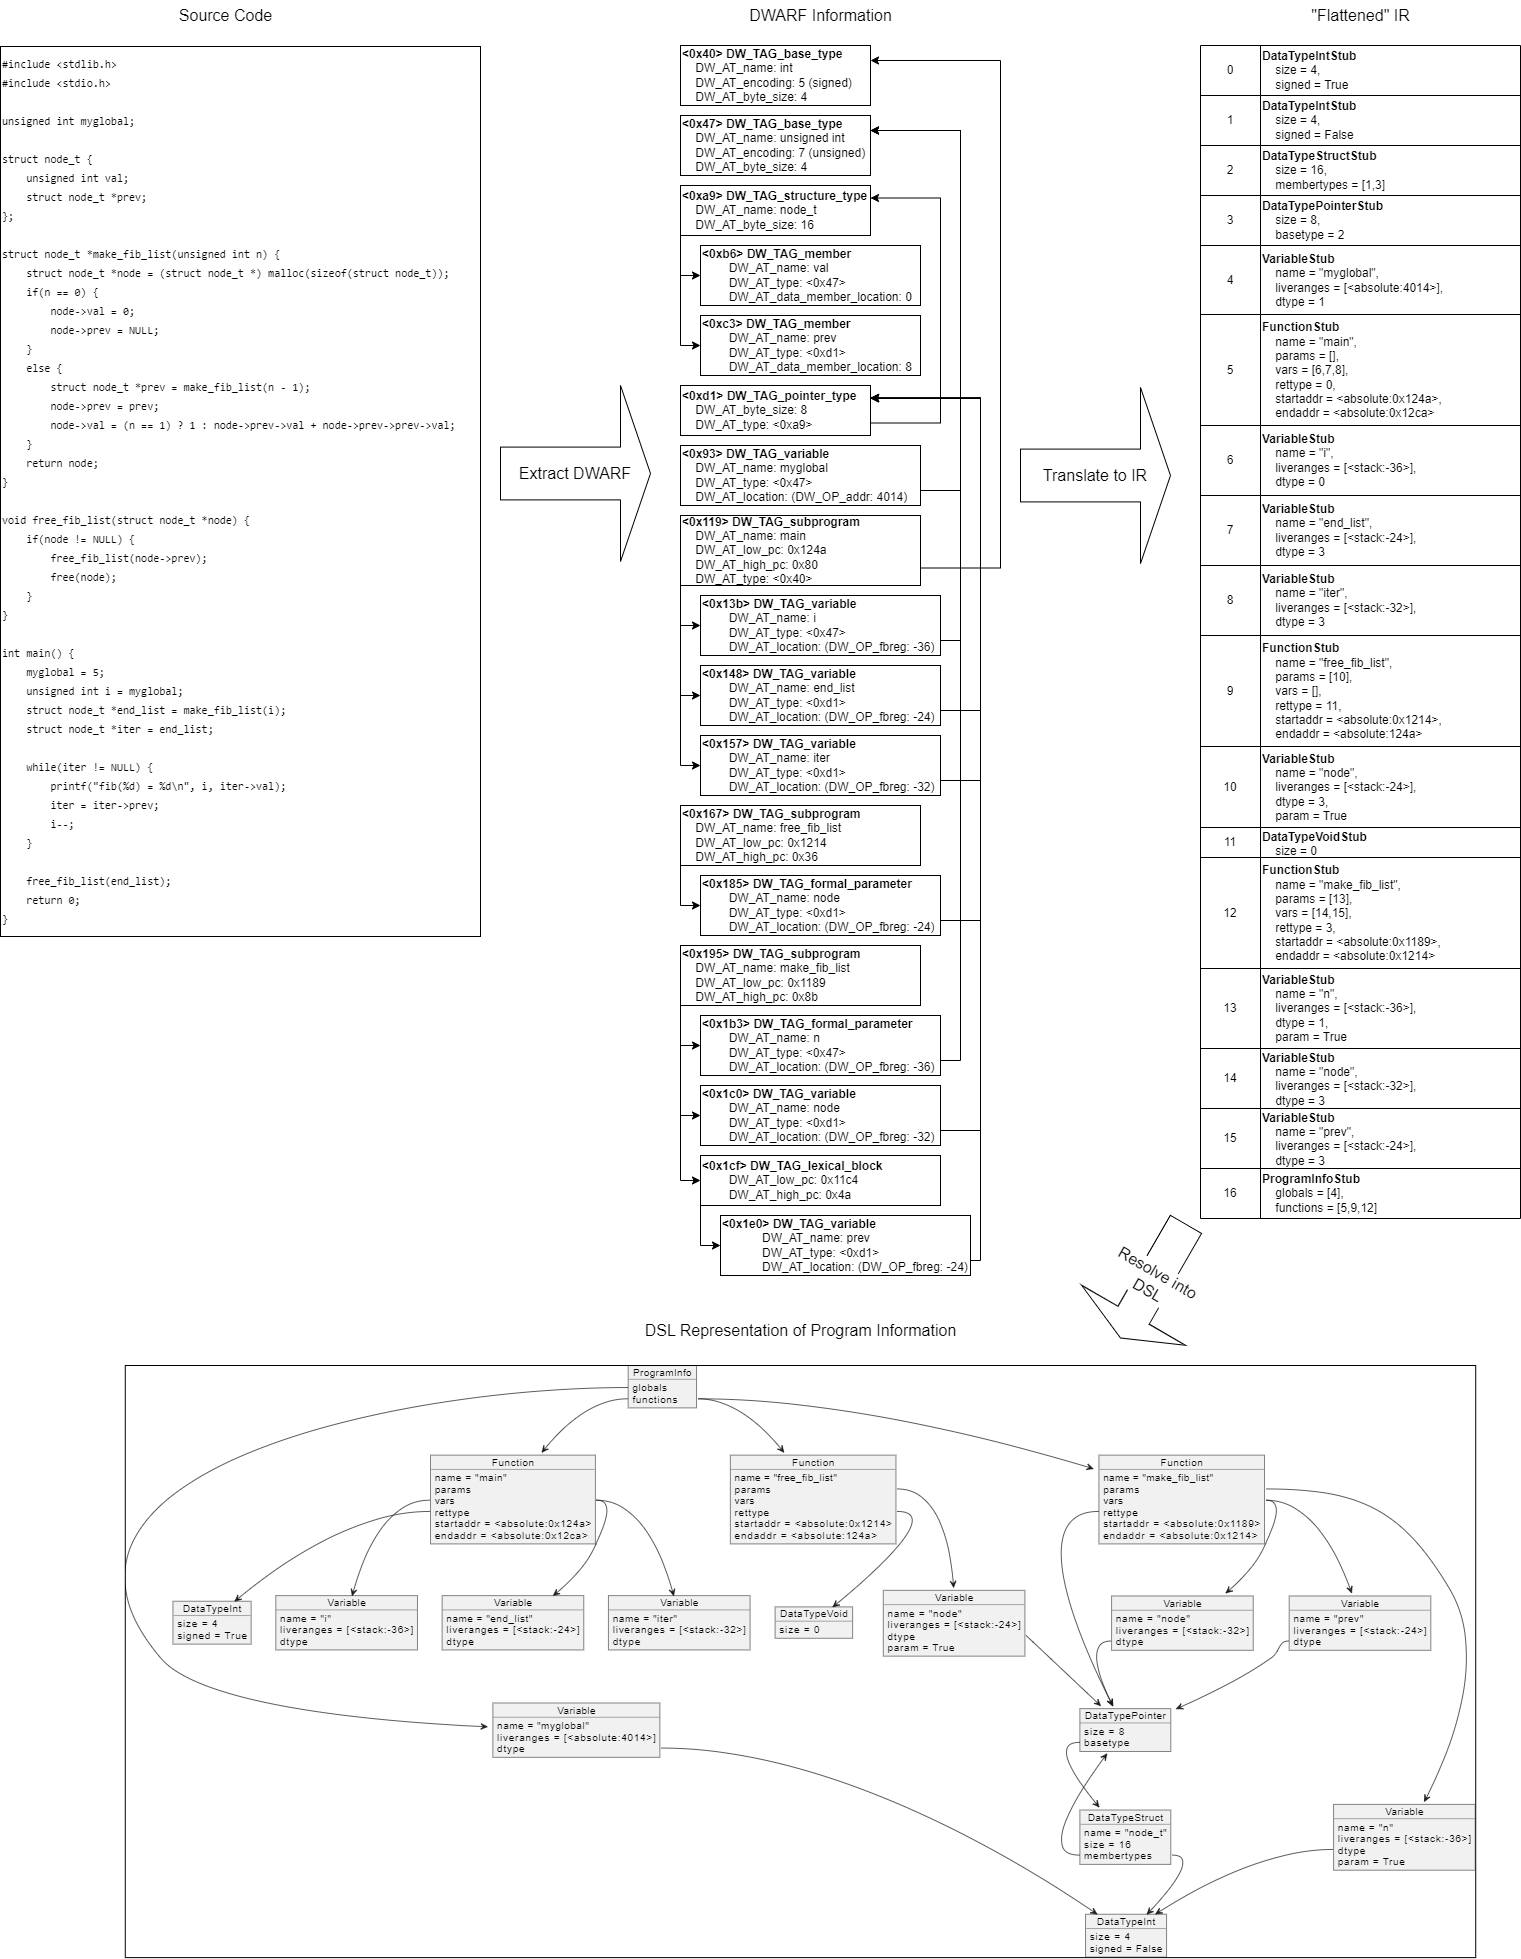
\includegraphics[width=\textwidth]{./figures/parse-dwarf.drawio.png}
%     \caption{An example of translating DWARF information into the DSL}
%     \label{fig:parse-dwarf}
% \end{figure*}

\subsection{Capturing Decompiler (Ghidra) Output Information}

In addition to capturing a ground-truth program representation in our DSL, we must construct a DSL representation of the program information obtained from a decompiler we wish to evaluate. Depending on the decompiler and the structure of its output, this process may take many forms, often involving querying APIs exposed by the decompiler framework. In all cases however, this shall involve defining a translation module from the decompiler output to the constructs defined in the DSL.

For our analysis of the Ghidra decompiler, we utilize the Ghidra scripting API to programmatically scrape and process information about the decompilation of target binary programs. The Ghidra scripting environment exposes its own collection of data structures and functions from which we obtain our information.

The strategy employed for the Ghidra translation is similar to that of our DWARF translation algorithm. We utilize the Ghidra API to obtain particular information about functions, variables, data types, and associated addresses gathered during the decompilation, and subsequently translate this information into the structure of our DSL. Of particular use to our translation logic is the \emph{DecompInterface} interface exposed by the Ghidra API.

\subsection{Comparison of Ground Truth and Decompiler Program Information}

With the ability to convert ground truth and decompiler (Ghidra) program information into our DSL, we formulate and implement a strategy to compare the two resulting \emph{ProgramInfo} objects. To achieve this, we create an extension of our DSL that defines data structures and functions for capturing comparison information at different levels.

\subsubsection{Data Type Comparison}

Given two \emph{DataType} objects and an offset between their start locations, we devise a method to capture nuanced information about the comparison of the data types.

\paragraph{Definitions}

We define the \emph{metatype} of a data type to be general "class" of the given data type. These metatypes include \emph{INT}, \emph{FLOAT}, \emph{POINTER}, \emph{ARRAY}, \emph{STRUCT}, \emph{UNION}, \emph{UNDEFINED}, \emph{VOID}, and \emph{FUNCTION\_PROTOTYPE}. We consider \emph{INT}, \emph{FLOAT}, \emph{POINTER}, \emph{UNDEFINED}, and \emph{VOID} to be \emph{primitive metatypes} since they cannot be decomposed further. \emph{ARRAY}, \emph{STRUCT}, and \emph{UNION} are considered \emph{complex metatypes} since these types are formed via the composition or aggregation of different members or subtypes. We consider the 'char' data type to be of the \emph{INT} metatype with size equal to one byte.

% [Figure: Ariste type lattice]
\begin{figure}[htb]
    \centering
    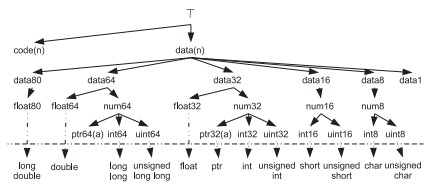
\includegraphics[width=\columnwidth]{./figures/ariste-type-lattice.png}
    \caption{The ARTISTE type lattice \cite{bib:artiste,bib:type-inference-executables}.}
    \label{fig:artiste-type-lattice}
\end{figure}

A \emph{primitive type lattice} \cite{bib:type-inference-executables} is used to hierarchically relate primitive data types based on their metatype, size, and signedness (if applicable). More general types are located higher in the lattice while more specific types are located closer to the leaves. A type lattice may be used to determine whether two primitive data types are equivalent or share a common parent type. Our framework leverages a modified version of the ARTISTE primitive type lattice defined in Caballero et. al \cite{bib:artiste} and shown in Figure \ref{fig:artiste-type-lattice}.

% [Figure: Subset relationship example(s)]

We next define a \emph{subset} relationship between two data types. For a given complex data type X and another data type Y with a given offset (possibly 0) between the location of X and Y in memory, Y is considered a \emph{subset} type of X if Y is equivalent to a "portion" of X, consistent with the offset between X and Y. For example, if X is an array, any sub-array or element of X such that elements are aligned and the element types are equivalent to X is considered a subset of X. If X is a struct or union, any sub-struct or member with proper alignment and equal constituent elements is considered a subset of X.

\paragraph{Comparison Logic}

Suppose we have two \emph{DataType} objects X (ground truth) and Y (decompiler) with offset k from the start of X to the start of Y. The goal is to compute the \emph{data type comparison level} for the given comparison. The possible values for the comparison level are as follows, from lowest equality to highest equality:

\begin{itemize}
    \item \emph{NO\_MATCH}: No relationship could be found between X and Y.
    \item \emph{SUBSET}: Y is a subset type of the complex type X.
    \item \emph{PRIMITIVE\_COMMON\_ANCESTOR}: In the primitive type lattice, Y is an ancestor of X. This indicates that the inferred type Y is a conservative (more general) form of the ground truth type X.
    \item \emph{MATCH}: All properties of X and Y match including metatype, size, and possibly subtypes (applicable to pointers, arrays, structs, and unions).
\end{itemize}

We first check the equality of X and Y. If X and Y are equal, we assign the \emph{MATCH} comparison code. In the case that X and Y are both primitive types, we attempt to compute their shared ancestor in the primitive type lattice. If Y is an ancestor (more general form) of X, we assign \emph{PRIMITIVE\_COMMON\_ANCESTOR}. If X is a complex type, we employ an algorithm to determine whether Y is a subset of X at offset k by recursively descending into constituent portions of X starting at offset k (sub-structs, sub-arrays, elements, members) and checking for equality with Y. If a subset relationship is found, we assign the \emph{SUBSET} compare level. In all other cases, we assign the \emph{NO\_MATCH} compare level.

\subsubsection{Variable (Varnode) Comparison}

There are two main contexts where variable comparison occurs. The first context is at the top level, where the set of ground-truth global variables is compared to the set of decompiler global variables. The second context for variable comparison is within the context of a function when we compare local variables between the ground-truth and the decompiler. In either case, comparing sets of variables starts with the decomposition of each \emph{Variable} object from the DSL into a set of \emph{Varnode} objects in our extended DSL.

A \emph{Varnode} ties a \emph{Variable} to a specific storage location and the range of PC addresses indicating when variable lives at that location. The varnodes for a given variable are directly computed from the variable's live ranges discussed previously. In unoptimized binaries, it is the case that a single \emph{Variable} shall decompose into a single \emph{Varnode}.

With each variable decomposed into its associated varnodes, we next partition the varnodes from each the ground-truth and the decompiler based on the "address space" in which they reside. These address spaces include the \emph{absolute} address space, the \emph{stack} address space, and the \emph{register offset} address space (for a given register). The \emph{stack} address space is a special case of the \emph{register offset} address space where the offset register is the base pointer which points to the base of the current stack frame.

For the set of varnodes in each address space, we first order them based on their offset within the address space. Next, we attempt to find overlaps between varnodes from the two sources based on their location and size. If an overlap occurs between two varnodes, we compute a data type comparison taking into account the offset between the start locations of the two varnodes. The data type comparison approach is described in the previous section.

Based on the overlap status and data type comparison of a ground-truth varnode X, one of the following \emph{varnode comparison levels} will be assigned:

\begin{itemize}
    \item \emph{NO\_MATCH}: X is not overlapped with any varnodes from the other source.
    \item \emph{OVERLAP}: X overlaps with one or more varnodes from the other space, but the data type comparisons are level \emph{NO\_MATCH}.
    \item \emph{SUBSET}: X overlaps with one or more varnodes and each of its compared varnodes has data type comparison level equal to \emph{SUBSET}. In other words, the compared varnode(s) make up a portion of X.
    \item \emph{ALIGNED}: For some varnode Y from the other source, X and Y share the same location and size in memory; however, the data types of X and Y do not match. The data types comparison could have any comparison level less than \emph{MATCH}.
    \item \emph{MATCH}: For some varnode Y from the other source, X and Y share the same location and size in memory, and their data types match exactly.
\end{itemize}

% [Figure: Varnode comparison levels derived from varnode recovery and data type comparison]
\begin{figure}[htb]
    \centering
    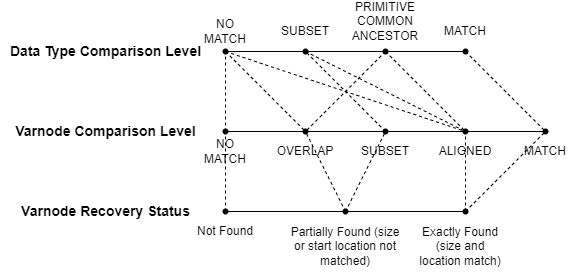
\includegraphics[width=\columnwidth]{./figures/varnode-levels.drawio.png}
    \caption{The derivation of varnode comparison level from varnode recovery status and data type comparison.}
    \label{fig:varnode-levels}
\end{figure}

\paragraph{Decomposed Variable Comparison}

The inference of variables with complex data types including structs, arrays, and unions proves to be a major challenge for decompilers. Recognizing this, we develop an approach to compare the sets of ground truth and decompiler variables (varnodes) in their most "decomposed" forms. An analysis of this sort helps to recognize how well a decompiler infers the primitive constituent components of complex variables. Furthermore, this allows us to recognize the aggressiveness and accuracy of complex variable synthesis from more primitive components.

% [Figure: Example of "decomposing" complex varnode]
\begin{figure*}[tb]
    \begin{subfigure}{0.25\textwidth}
        \centering
        \begin{Verbatim}[frame=single]
typedef struct {
    int day;
    int month;
    int year;
} Date;

typedef struct {
    char* name;
    int ssn;
    float height;
    float weight;
    Date dob;
} Person;

Person people[2];
        \end{Verbatim}
        \caption{The definition of a high-level variable.}
        \label{fig:decompose-src}
    \end{subfigure}
    \hfill
    \begin{subfigure}{0.75\textwidth}
        \scalebox{0.35}[0.4]{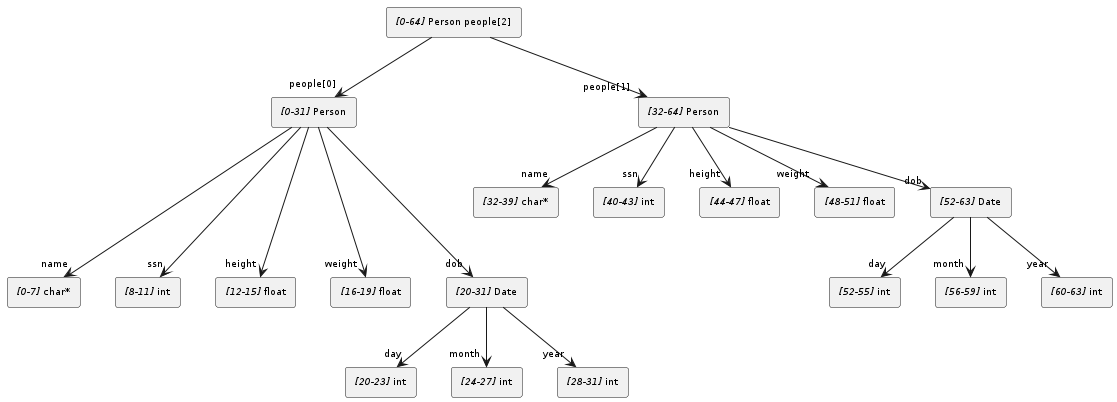
\includegraphics{./figures/decompose.png}}
        \caption{The decomposition of a high-level varnode into primitive components.}
        \label{fig:decompose-tree}
    \end{subfigure}
    \caption{An example of the recursive decomposition of a high-level varnode.}
    \label{fig:decompose}
\end{figure*}

We first implement an approach to recursively strip away the "complex layers" of a varnode to its most primitive decomposition. This primitive decomposition produces a set of one or more primitive varnodes as they would appear in memory. For example, an array of elements is broken down into a set of its elements (decomposed recursively). A struct is broken down into a set of varnodes associated with each of its members (decomposed recursively). Unions present a special case since the members share a common, overlapping region of memory. Hence, to decompose a union, we transform it into an \emph{UNDEFINED} primitive type with the same size as the union.

We apply this primitive decomposition to each varnode in the sets of ground truth and decompiler varnodes. With the two sets of decomposed varnodes, we leverage the same variable comparison approach described previously to compare the varnodes in these sets. The resulting comparison information is treated as a separate analysis from the unaltered varnode sets.

% [Figure: An example of varnode comparisons on the stack]
% \begin{figure*}[tb]
%     \centering
%     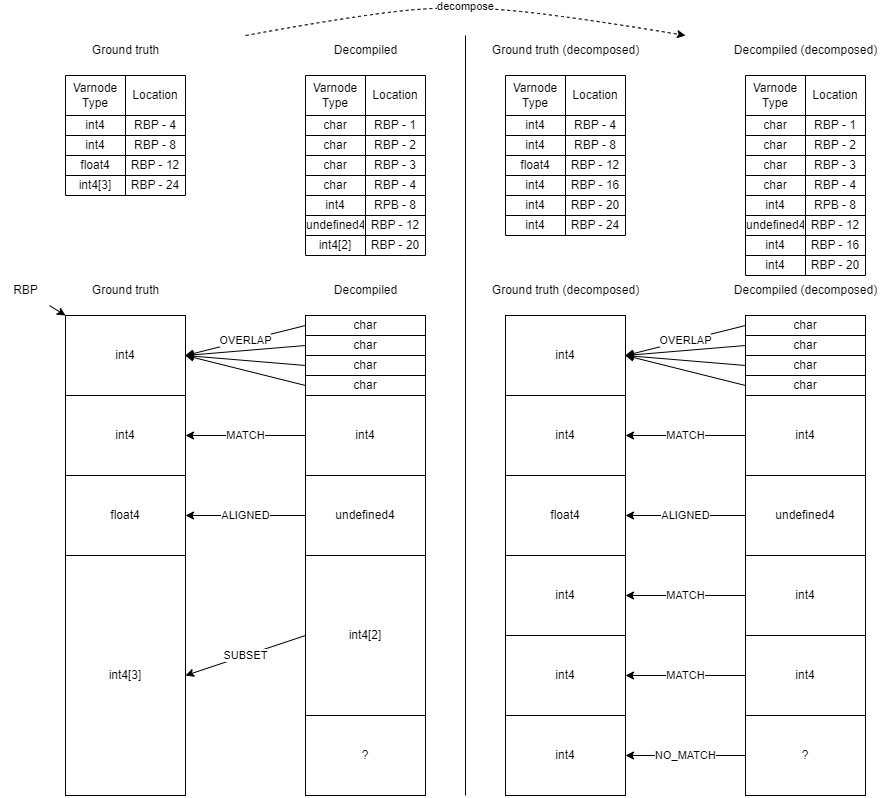
\includegraphics[width=\textwidth]{./figures/stack-comparison.drawio.png}
%     \caption{An example of varnode comparisons between ground truth and decompiler varnodes for a given stack frame.}
%     \label{fig:stack-comparison}
% \end{figure*}

\subsubsection{Function Comparison}

The first step in function comparison is to determine whether each ground-truth function is found by the decompiler. We first order the functions from each source by the start PC address of the function. Next, we attempt to match the functions from the two sources based on start address. Any functions from the ground-truth that are not matched by a decompiler function are considered "missed". For any missed functions, we consider its associated parameters, local variables, and data types to also be "missed".

For each "matched" function based on start PC address, we compute and store information including the return type comparison, parameter comparisons, and local variable comparisons. These sub-comparisons leverage the data type and variable  (varnode) comparison techniques described previously.


\section{\uppercase{Evaluation}} \label{sec:evaluation}

To demonstrate our evaluation framework, we target the Ghidra decompiler (version 10.2). We use the GNU Core Utilities programs (version 9.1) as our set of benchmarks. For each of the benchmark programs, we evaluate the accuracy of Ghidra decompilation with the program compiled in three ways: (1) stripped, (2) standard (not stripped, no debugging symbols), and (3) DWARF debug symbols included. We use the results from each of these cases to discern how the amount of information included in the binary affects the Ghidra decompiler's inference accuracy. To limit the scope of our analysis, we only consider unoptimized binaries. We use the GCC compiler (version 11.1.0) to compile the benchmark programs. The architecture and operating system of the testing machine are x86-64 and Ubuntu Linux (version 20.04), respectively. Figure \ref{fig:evaluation-process} illustrates our process for gathering evaluation metrics on an individual benchmark program under each of the compilation conditions.

\begin{figure}[htb]
    \centering
    % \scalebox{0.2}{
    %     \input{./figures/evaluation-process.latex}
    % }
    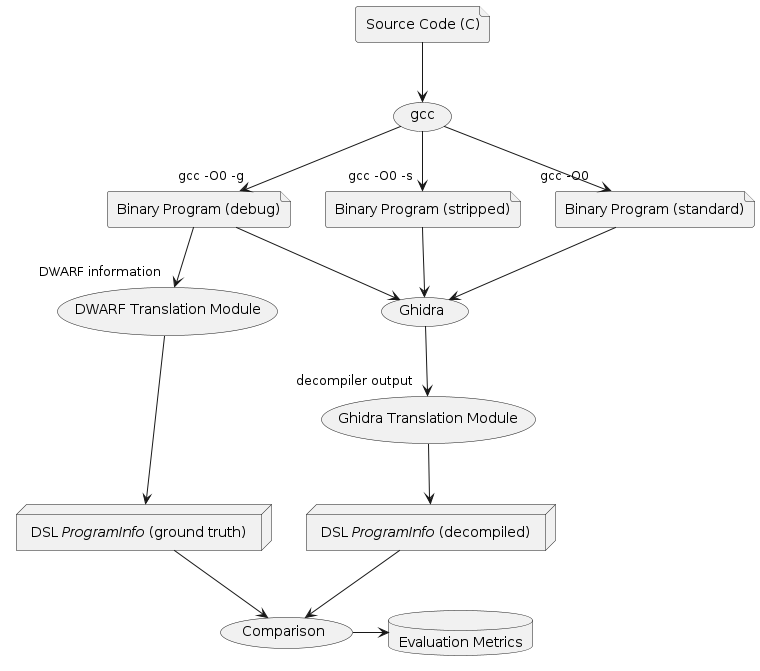
\includegraphics[width=\columnwidth]{./figures/evaluation-process.png}
    \caption{The process used to gather evaluation metrics on the Ghidra decompiler for a given benchmark program.}
    \label{fig:evaluation-process}
\end{figure}

\subsection{Function Recovery}

\begin{table}[htb]
\centering
\caption{A summary of function recovery by compilation case.}
\label{table:opts-functions-summary}
\begin{tabular}{lp{0.15\columnwidth}p{0.15\columnwidth}p{0.15\columnwidth}p{0.15\columnwidth}p{0.15\columnwidth}}
\toprule
{} &  Ground truth functions &  Functions found &  Functions missed &  Functions recovery fraction \\
\midrule
strip    &                   18139 &            18139 &                 0 &                       1.0000 \\
standard &                   18139 &            18139 &                 0 &                       1.0000 \\
debug    &                   18139 &            18135 &                 4 &                       0.9998 \\
\bottomrule
\end{tabular}
\end{table}


Table \ref{table:opts-functions-summary} shows the summarization of the recovery statistics accumulated over all benchmark programs. We find that over the 18139 functions present in the ground truth, the stripped and standard compilation cases produce 100\% function recovery while the debug case fails to recover four functions, resulting in a 99.9\% recovery rate. Upon futher examination, we find that all four functions missed are from the \emph{factor} program.

To determine the cause of the missed functions, we further investigate the Ghidra decompilation of \emph{factor} and find that each of the missed functions results in a decompilation error, "Low-level Error: Unsupported data-type for ResolveUnion". This indicates that an error occurred when attempting to resolve a union data type within the decompilation of these functions. Since this error only occurs in the debug compilation case, it is clear that Ghidra's parsing and interpretation of DWARF information contributes to this error. This same union data type causing the error is successfully captured and represented in our ground truth program information and, thus, this is likely a bug within Ghidra's resolution logic.

In summary, we see that Ghidra successfully finds all functions for all compilation configurations. However, in the debug case, Ghidra's attempt to interpret and utilize DWARF information to resolve a union data type in the \emph{factor} program results in a decompiler error for four functions. This error indicates a bug in Ghidra's DWARF parsing or union resolution logic.

\subsection{High-Level Variable (Varnode) Recovery}

To evaluate the variable (varnode) recovery accuracy of the Ghidra decompiler, we first measure the inference performance of high-level varnodes, including varnodes with complex and aggregate types such as arrays, structs, and unions. We further measure the varnode inference accuracy by metatype to decipher which of the metatypes are most and least accurately inferred by the decompiler. This analysis is performed under each compilation configuration (stripped, standard, and debug).

In all our varnode evaluation tables, the \emph{Varnode comparison score} metric is defined as follows: For each \emph{varnode comparison level}, we first linearly assign an integer representing the strength of the varnode comparison (\emph{NO\_MATCH} = 0, \emph{OVERLAP} = 1, \emph{SUBSET} = 2, \emph{ALIGNED} = 3, \emph{MATCH} = 4). We then normalize these scores to fall within the range zero to one. Then, for each ground truth varnode, we compute this normalized score. We take the average score over all ground truth varnodes to obtain the resulting metric. This metric approximates how well, on average, the decompiler infers the ground truth varnodes.

\begin{table*}[tb]
\centering
\caption{A summary of high-level varnode recovery by compilation case.}
\label{table:opts-varnodes-summary}
\begin{tabular}{lp{1.50cm}p{1.33cm}p{1.33cm}p{1.33cm}p{1.33cm}p{1.33cm}p{1.33cm}p{1.33cm}p{1.33cm}}
\toprule
{} & {Varnodes matched @ level NO\_MATCH} & {Varnodes matched @ level OVERLAP} & {Varnodes matched @ level SUBSET} & {Varnodes matched @ level ALIGNED} & {Varnodes matched @ level MATCH} & {Varnode comparison score} & {Varnodes fraction partially recovered} & {Varnodes fraction exactly recovered} \\
\midrule
strip    &                                               1000 &                                             1662 &                                            1001 &                                            18570 &                                          12550 &                                    0.788 &                                              0.971 &                                              0.361 \\
standard &                                                249 &                                             1450 &                                             613 &                                            19029 &                                          13442 &                                    0.816 &                                              0.993 &                                              0.386 \\
debug    &                                                 23 &                                               52 &                                              24 &                                                7 &                                          34677 &                                    0.998 &                                              0.999 &                                              0.997 \\
\bottomrule
\end{tabular}
\end{table*}


In Table \ref{table:opts-varnodes-summary}, we show the high-level varnode recovery metrics for each of the compilation conditions, aggregated from each of the benchmark programs. We find that Ghidra at least partially infers 97.2\%, 99.3\%, and 99.6\% and precisely infers 36.1\%, 38.6\%, and 99.7\% of high-level varnodes for each for the stripped, standard, and debug compilation cases, respectively. In addition, the varnode comparison scores for each compilation case are 0.788, 0.816, and 0.998, respectively. These metrics indicate that the standard compilation case slightly outperforms the stripped case in varnode inference while the debug compilation case results in significant improvements over both the stripped and standard cases, particularly in exact varnode recovery.

\begin{table*}[tb]
\centering
\caption{A summary of high-level varnode recovery by compilation case and metatype.}
\label{table:opts-varnodes-summary-metatypes}
\begin{tabular}{lp{1.50cm}p{1.50cm}p{1.33cm}p{1.33cm}p{1.33cm}p{1.33cm}p{1.33cm}p{1.33cm}p{1.33cm}}
\toprule
      &       & {Varnodes matched @ level NO\_MATCH} & {Varnodes matched @ level OVERLAP} & {Varnodes matched @ level SUBSET} & {Varnodes matched @ level ALIGNED} & {Varnodes matched @ level MATCH} & {Varnode comparison score} & {Varnodes fraction partially recovered} & {Varnodes fraction exactly recovered} \\
\midrule
\multirow{6}{*}{strip} & INT &                                                 66 &                                               48 &                                               0 &                                            12204 &                                           8681 &                                    0.850 &                                              0.997 &                                              0.413 \\
      & FLOAT &                                                  0 &                                               56 &                                               0 &                                              113 &                                             22 &                                    0.632 &                                              1.000 &                                              0.115 \\
      & POINTER &                                                 53 &                                                4 &                                               0 &                                             5834 &                                           3513 &                                    0.839 &                                              0.994 &                                              0.374 \\
      & ARRAY &                                                729 &                                              597 &                                             565 &                                               19 &                                            228 &                                    0.315 &                                              0.659 &                                              0.107 \\
      & STRUCT &                                                152 &                                              955 &                                             432 &                                              390 &                                            106 &                                    0.419 &                                              0.925 &                                              0.052 \\
      & UNION &                                                  0 &                                                2 &                                               4 &                                               10 &                                              0 &                                    0.625 &                                              1.000 &                                              0.000 \\
\cline{1-10}
\multirow{6}{*}{standard} & INT &                                                 23 &                                               48 &                                               0 &                                            12248 &                                           8680 &                                    0.851 &                                              0.999 &                                              0.413 \\
      & FLOAT &                                                  0 &                                               56 &                                               0 &                                              113 &                                             22 &                                    0.632 &                                              1.000 &                                              0.115 \\
      & POINTER &                                                 44 &                                                4 &                                               0 &                                             5836 &                                           3520 &                                    0.840 &                                              0.995 &                                              0.374 \\
      & ARRAY &                                                181 &                                              578 &                                             352 &                                               45 &                                            982 &                                    0.625 &                                              0.915 &                                              0.459 \\
      & STRUCT &                                                  1 &                                              762 &                                             257 &                                              777 &                                            238 &                                    0.560 &                                              1.000 &                                              0.117 \\
      & UNION &                                                  0 &                                                2 &                                               4 &                                               10 &                                              0 &                                    0.625 &                                              1.000 &                                              0.000 \\
\cline{1-10}
\multirow{6}{*}{debug} & INT &                                                 13 &                                               27 &                                               0 &                                                4 &                                          20955 &                                    0.998 &                                              0.999 &                                              0.998 \\
      & FLOAT &                                                  0 &                                                0 &                                               0 &                                                0 &                                            191 &                                    1.000 &                                              1.000 &                                              1.000 \\
      & POINTER &                                                  3 &                                                0 &                                               0 &                                                1 &                                           9400 &                                    1.000 &                                              1.000 &                                              1.000 \\
      & ARRAY &                                                  5 &                                               17 &                                              24 &                                                0 &                                           2092 &                                    0.986 &                                              0.998 &                                              0.978 \\
      & STRUCT &                                                  2 &                                                8 &                                               0 &                                                0 &                                           2025 &                                    0.996 &                                              0.999 &                                              0.995 \\
      & UNION &                                                  0 &                                                0 &                                               0 &                                                2 &                                             14 &                                    0.969 &                                              1.000 &                                              0.875 \\
\bottomrule
\end{tabular}
\end{table*}


In Table \ref{table:opts-varnodes-summary-metatypes}, we show the inference performance of high-level varnodes broken down by the metatype for each compilation configuration. From the stripped and standard compilation cases, we observe that varnodes with metatype \emph{INT} are most accurately recovered when considering varnode comparison score, fraction partially recovered, and fraction exactly recovered. In the stripped case, the inference of \emph{ARRAY} varnodes shows the worst performance with a varnode comparison score of 0.315. In the standard case, varnodes with metatype \emph{STRUCT} are least accurately recovered with a varnode comparison score of 0.560, followed closely by \emph{ARRAY} and \emph{UNION}. We see that, for both the stripped and standard compilation cases, the complex (aggregate) metatypes, \emph{ARRAY}, \emph{STRUCT}, and \emph{UNION}, show the lowest recovery accuracy with respect to varnode comparison score. Among the primitive metatypes, \emph{FLOAT} shows the worst recovery metrics for these two compilation cases.

The debug compilation case demonstrates high relative recovery accuracy across varnodes of all metatypes when compared to the stripped and standard cases. Of the primitive metatypes, varnodes of the \emph{FLOAT} metatype are perfectly recovered while varnodes of the \emph{INT} and \emph{POINTER} metatypes show exact recovery percentages of 99.8\% and 99.9\%, respectively. The complex (aggregate) metatypes, on average, display slightly lower recovery metrics than the primitive metatypes in the debug compilation case. The \emph{ARRAY} metatype reveals the worst varnode comparison score at 0.986. The \emph{UNION} metatype demonstrates the lowest exact match percentage at 87.5\%.

\subsection{Decomposed Variable (Varnode) Recovery}

In this section, we repeat a similar varnode recovery analysis over all varnodes; however, we first recursively decompose each varnode into a set of primitive varnodes (see Section \ref{sec:methodology}). We perform this analysis over all benchmarks for each of the three compilation cases.

\begin{table*}[tb]
\centering
\caption{A summary of decomposed varnode recovery by compilation case.}
\label{table:opts-varnodes-summary-decomposed}
\begin{tabular}{lp{1.50cm}p{1.33cm}p{1.33cm}p{1.33cm}p{1.33cm}p{1.33cm}p{1.33cm}p{1.33cm}p{1.33cm}}
\toprule
{} & {Varnodes matched @ level NO\_MATCH} & {Varnodes matched @ level OVERLAP} & {Varnodes matched @ level SUBSET} & {Varnodes matched @ level ALIGNED} & {Varnodes matched @ level MATCH} & {Varnode comparison score} & {Varnodes fraction partially recovered} & {Varnodes fraction exactly recovered} \\
\midrule
strip    &                                             139776 &                                            31280 &                                               0 &                                           231267 &                                         131593 &                                    0.586 &                                              0.738 &                                              0.246 \\
standard &                                              40187 &                                            56605 &                                               0 &                                           303527 &                                         133597 &                                    0.703 &                                              0.925 &                                              0.250 \\
debug    &                                              10547 &                                              128 &                                               0 &                                                5 &                                         523236 &                                    0.980 &                                              0.980 &                                              0.980 \\
\bottomrule
\end{tabular}
\end{table*}


Similar to the high-level varnode analysis, we show the inference of the decomposed varnodes for each benchmark and for each compilation configuration in Table \ref{table:opts-varnodes-summary-decomposed}. Naturally, we expect to see lower recovery metrics compared to the high-level varnode analysis since each complex varnode is now analyzed as a set of its constituent parts. Hence, a single "missed" high-level varnode is translated into a set of primitive varnodes, each "missed" in this analysis. We find this hypothesis to hold true across all compilation cases as each the varnode comparison score, varnodes fraction partially recovered, and varnodes fraction exactly recovered show lower values than in the high-level analysis. We see that the decomposed varnode comparison scores for the strip, standard, and debug compilation cases are 0.586, 0.703, and 0.980, respectively. The varnodes fraction partially recovered are 73.8\%, 92.5\%, and 98.0\% while the varnodes fraction exactly recovered are 24.7\%, 25.0\%, and 98.0\% across the compilation cases, respectively. Interestingly, in the stripped compilation case, we find that the number of "missed" decomposed varnodes (139937) exceeds the number of "exactly matched" decomposed varnodes (131719). This is largely due to the quantity of high-level \emph{ARRAY} and \emph{STRUCT} varnodes that are missed in the stripped case.

\begin{table*}[tb]
\centering
\caption{A summary of decomposed varnode recovery by compilation case and primitive metatype.}
\label{table:opts-varnodes-summary-metatypes-decomposed}
\begin{tabular}{lp{1.50cm}p{1.50cm}p{1.33cm}p{1.33cm}p{1.33cm}p{1.33cm}p{1.33cm}p{1.33cm}p{1.33cm}}
\toprule
      &         & {Varnodes matched @ level NO\_MATCH} & {Varnodes matched @ level OVERLAP} & {Varnodes matched @ level SUBSET} & {Varnodes matched @ level ALIGNED} & {Varnodes matched @ level MATCH} & {Varnode comparison score} & {Varnodes fraction partially recovered} & {Varnodes fraction exactly recovered} \\
\midrule
\multirow{3}{*}{strip} & INT &                                             132910 &                                            28812 &                                               0 &                                           217923 &                                         125159 &                                    0.586 &                                              0.737 &                                              0.248 \\
      & FLOAT &                                                 72 &                                               73 &                                               0 &                                              103 &                                             22 &                                    0.435 &                                              0.733 &                                              0.081 \\
      & POINTER &                                               6725 &                                             2057 &                                               0 &                                            13208 &                                           6332 &                                    0.591 &                                              0.763 &                                              0.224 \\
\cline{1-10}
\multirow{3}{*}{standard} & INT &                                              40017 &                                            46846 &                                               0 &                                           290436 &                                         127505 &                                    0.707 &                                              0.921 &                                              0.253 \\
      & FLOAT &                                                  0 &                                              145 &                                               0 &                                              103 &                                             22 &                                    0.502 &                                              1.000 &                                              0.081 \\
      & POINTER &                                                132 &                                             9245 &                                               0 &                                            12955 &                                           5990 &                                    0.636 &                                              0.995 &                                              0.211 \\
\cline{1-10}
\multirow{3}{*}{debug} & INT &                                              10533 &                                              124 &                                               0 &                                                4 &                                         494143 &                                    0.979 &                                              0.979 &                                              0.979 \\
      & FLOAT &                                                  0 &                                                0 &                                               0 &                                                0 &                                            270 &                                    1.000 &                                              1.000 &                                              1.000 \\
      & POINTER &                                                 14 &                                                2 &                                               0 &                                                1 &                                          28305 &                                    0.999 &                                              1.000 &                                              0.999 \\
\bottomrule
\end{tabular}
\end{table*}


We partition the decomposed varnodes by metatype and show these results in Table \ref{table:opts-varnodes-summary-metatypes-decomposed}. The table shows that the stripped and standard compilation cases demostrate the poorest inference performance in terms of varnode comparison score for varnodes of metatype \emph{FLOAT}. However, we find that the percentage of "missed" \emph{INT} varnodes is worse than that of \emph{FLOAT} in the standard and debug compilation cases, and is nearly the same in the stripped case. This may be explained by the prevalence of integer (or character) arrays in the Coreutils benchmark programs when compared to other array types. Recovery accuracy of the \emph{POINTER} metatype is comparable to the \emph{INT} metatype across the three compilation cases.

\subsection{Data Bytes Recovery}

Following from our varnode inference analysis, we next assess the accuracy of the Ghidra decompiler with regards to the total number of data bytes recovered across all varnodes. This analysis provides an important perspective on data recovery as the size of an improperly inferred varnode may result in a wide range in the number of misinferred bytes. For example, a large array and a single character are each represented by a varnode, but the quantity of data present in the array is much greater than that of a character. Hence, it is important to capture this nuanced view of data recovery.

\begin{table}[htb]
\centering
\caption{A summary of data bytes recovery by compilation case.}
\label{table:opts-bytes-summary}
\begin{tabular}{lp{0.15\columnwidth}p{0.15\columnwidth}p{0.15\columnwidth}p{0.15\columnwidth}p{0.15\columnwidth}}
\toprule
{} &  Ground truth data bytes &  Bytes found &  Bytes missed &  Bytes recovery fraction \\
\midrule
strip    &                  1183691 &       725144 &        458547 &                    0.613 \\
standard &                  1183691 &       954105 &        229586 &                    0.806 \\
debug    &                  1183691 &      1177221 &          6470 &                    0.995 \\
\bottomrule
\end{tabular}
\end{table}


In Table \ref{table:opts-bytes-summary}, we show the aggregated data bytes recovery metrics across the benchmark programs for each compilation case. We see that Ghidra recovers 61.3\%, 80.6\%, and 99.5\% of data bytes in the stripped, standard, and debug compilation cases, respectively.

\subsection{Array Inference Accuracy}

The last major analysis we perform targets the array inference accuracy of the Ghidra decompiler. We aim to measure metrics regarding the total number of arrays inferred, the length and size discrepancies of compared arrays, and the similarity of element types of compared arrays. The descriptions of the metrics are as follows:
\begin{itemize}
    \item \emph{Ground truth varnodes (metatype=ARRAY)}: The number of ground truth varnodes with metatype of ARRAY.
    \item \emph{Array comparisons}: The number of array comparisons made when comparing the ground truth with the decompiler. The decompiler may infer 0 or more array varnodes for each given ground truth array varnode.
    \item \emph{Array varnodes inferred as array}: This measures how many ground truth array varnodes are compared to at least one decompiler-inferred array varnode.
    \item \emph{Array varnodes inferred as array fraction}: Equivalent to \emph{Array varnodes inferred as array} divided by \emph{Ground truth varnodes (metatype=ARRAY)}. This expresses the fraction of ground truth array varnodes that are associated with at least one decompiler array inference.
    \item \emph{Array length (elements) average error}: For each array comparison, we find the absolute difference in the number of elements inferred by the decompiler as compared to the ground truth. We then average these differences over all array comparisons to arrive at this metric.
    \item \emph{Array length (elements) average error ratio}: For each array comparison, we first find the absolute difference in the number of elements inferred by the decompiler as compared to the ground truth. We then divide this error by the length of the ground truth array to get the error as a ratio of the array size. The average of these ratios over all array comparisons produces this metric.
    \item \emph{Array size (bytes) average error}: This metric is similar to \emph{Array length (elements) average error} but measures the error in bytes instead of number of elements.
    \item \emph{Array size (bytes) average error ratio}: This metric is similar to \emph{Array length (elements) average error ratio} but computes the error in bytes instead of array elements.
    \item \emph{Array dimension match score}: This metric is the number of array comparisons where the decompiler inferred the correct number of dimensions divided by the total number of array comparisons.
    \item \emph{Array average element type comparison score}: Each \emph{data type comparison level} is first mapped to an integer as follows: \emph{NO\_MATCH} = 0, \emph{SUBSET} = 1, \emph{PRIMITIVE\_COMMON\_ANCESTOR} = 2, \emph{MATCH} = 3. We then normalize these values such that the range is scaled from 0 to 1. We refer to this as the \emph{data type comparison score}. Then, for each array comparison, we compute the \emph{data type comparison score} and subsequently average the scores across all array comparisons to generate this metric.
\end{itemize}

We perform our analysis across the benchmarks and for each compilation configuration, resuling in the data present in Table \ref{table:opts-array-comparisons-summary}.

\begin{table*}[tb]
\centering
\caption{A summary of array recovery by compilation case.}
\label{table:opts-array-comparisons-summary}
\begin{tabular}{lp{1.09cm}p{1.09cm}p{1.09cm}p{1.09cm}p{1.09cm}p{1.09cm}p{1.09cm}p{1.09cm}p{1.09cm}p{1.09cm}p{1.09cm}}
\toprule
{} & {Ground truth array varnodes} & {Array comparisons} & {Array varnodes inferred as array} & {Array varnodes inferred as array fraction} & {Array length (elements) average error} & {Array length (elements) average error ratio} & {Array size (bytes) average error} & {Array size (bytes) average error ratio} & {Array dimension match score} & {Array average element type comparison score} \\
\midrule
strip    &                                        2138 &                               823 &                                              774 &                                              0.362 &                                            134.695 &                                              2.845 &                                          458.575 &                                              0.912 &                                       0.979 &                                              0.781 \\
standard &                                        2138 &                              1579 &                                             1530 &                                              0.716 &                                            151.156 &                                              5.442 &                                          239.023 &                                              0.475 &                                       0.975 &                                              0.670 \\
debug    &                                        2138 &                              2226 &                                             2128 &                                              0.995 &                                              9.416 &                                              0.110 &                                            9.416 &                                              0.110 &                                       1.000 &                                              1.000 \\
\bottomrule
\end{tabular}
\end{table*}


Across all benchmarks, there are 2138 ground truth arrays present. For each the stripped, standard, and debug compilation cases, the number of ground truth arrays recognized as arrays by the decompiler are 774 (36.2\%), 1530 (71.6\%), and 2128 (99.5\%), respectively. We see that the numbers of array comparisons for each compilation case are greater than these metrics indicating that Ghidra infers some ground truth arrays to be more than one array.

From the array comparisons, we observe that the average absolute differential in array length (number of elements) for the stripped, standard, and debug compilation cases are 134.7, 151.2, and 9.4, respectively. When scaling these errors with respect to the length of the ground truth arrays in the comparisons, the error ratios are 2.84, 5.44, and 0.11 for the compilation cases, respectively. This reveals that, in the debug case for example, the lengths of decompiler-inferred arrays are off by an average of 9.4 elements and roughly 11\% (greater or less than) of the size of the ground truth arrays they are compared to. These metrics, however, fail to capture whether the decompiler-inferred array has element types of the correct length. Thus, a similar analysis on the size (number of bytes) errors yields errors and error ratios of 458.6 (0.91), 239 (0.47), and 9.41 (0.11) for each compilation case, respectively. This, for example, shows that arrays inferred in the standard compilation case have an average absolute byte differential of 239 and a relative error of 47\% compared to the size of the ground truth array they are compared to.

In this analysis, we also capture a measure of the array dimension match score for each compilation case. This metric measures the fraction of array comparisons where the decompiler-inferred array has the same dimensionality (one-dimensional, two-dimensional, etc.) as the ground truth array. The stripped and standard compilation cases display dimensionality match ratios of greater than 97.4\%, while the debug case shows 100\% dimensionality inference accuracy.

The last portion of our array recovery analysis focuses on the element type inference accuracy of the decompiler-inferred arrays when compared to the element types of the ground truth arrays. We compute a data type comparison score between the element types from each array comparison and average these across all array comparisons derived from our benchmark programs. This data type comparison score is similar in concept to the varnode comparison score and is described in Section \ref{sec:methodology}. We find that decompiler-inferred arrays in the stripped, standard, and debug compilation cases show 0.781, 0.670, and 0.999 average element type comparison scores, respectively. The better performance demonstrated in the stripped case compared to the standard case appears to be a data artifact resulting from fewer array comparisons present in the stripped analysis.

\subsection{Debug Compilation Case Discussion}

Upon examination of our results, the reader may wonder why the debug compilation case does not produce 100\% recovery for varnodes and data bytes across all benchmarks. The same DWARF debugging information used to generate the ground truth program information is also provided to the Ghidra decompiler in this case and therefore, theoretically, Ghidra should be able to precisely capture the same program information.

We explore the causes of misses and partial misses in the debug case across the benchmark programs and find that Ghidra possesses a major limitation in expressing local variables declared in lexical scopes below the top level of a function. A compiler such as GCC may reuse stack address space for variables associated with disjoint (non-overlapping and non-nested) lexical scopes. This is a problem for the Ghidra decompiler as we observe that all variable declarations are placed at the top level of the function, ultimately preventing these scope-specific variables from being precisely captured. From our manual analysis of the decompiled benchmark programs, we find that this is the cause of the majority of partially missed variables and data bytes in the debug compilation case. This limitation affects the stripped and standard compilation cases as well. We consider this to be a shortcoming and an area of future improvement for the Ghidra decompiler.

% [Figure: Ghidra missing variable in 2nd scope]
% \begin{figure*}[tb]
%     \centering
%     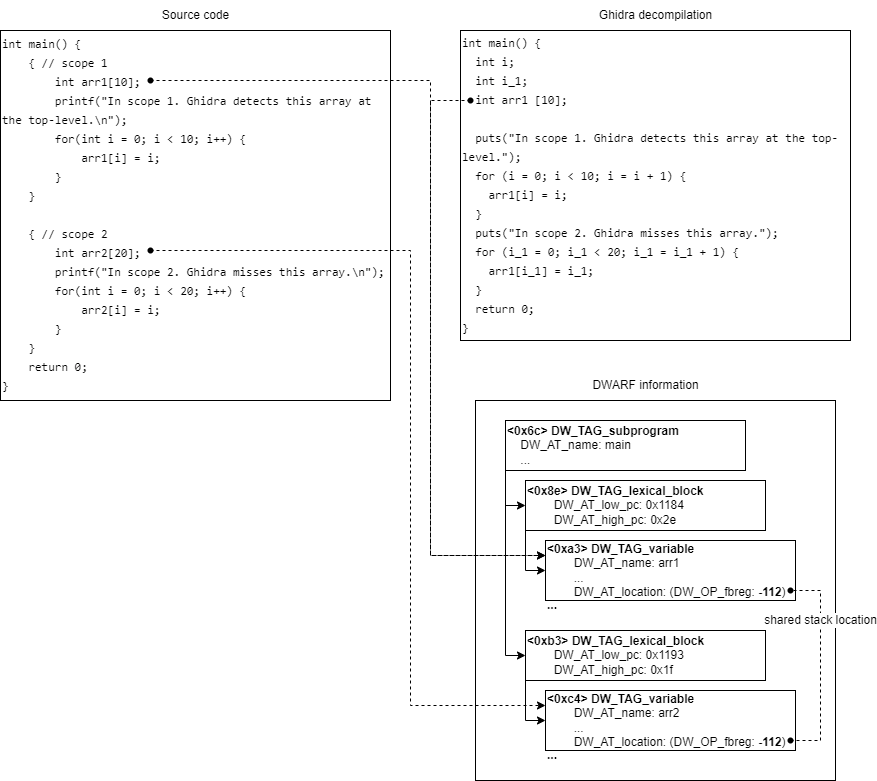
\includegraphics[width=\textwidth]{./figures/ghidra-miss-scopes.drawio.png}
%     \caption{An example of the Ghidra decompiler missing the second of two scope-specific variables that share stack space.}
%     \label{fig:ghidra-miss-scopes}
% \end{figure*}

\section{\uppercase{Conclusion}} \label{sec:conclusion}

\subsection{Contributions}

The three key contributions of this work are as follows:
\begin{enumerate}
    \item We develop a novel framework for evaluating decompiler tools based on the recovery accuracy of high-level program constructs, including functions, variables, and data types. This framework includes a domain-specific language (DSL), developed in Python, to represent and compare sources of high-level program information and their association with binary-level information. In addition, we devise quantitative metrics for expressing the recovery accuracy of high-level program constructs.
    \item We leverage our framework to perform an in-depth evaluation of the Ghidra decompiler with respect to high-level function, variable, and data type recovery. This evaluation is performed over the GNU Core Utilities programs under three compilation conditions.
    \item From our evalution of Ghidra, we discover and discuss the implications of two key issues present in the Ghidra decompiler.
\end{enumerate}

\subsection{Limitations}

The primary limitation of our framework in its current state is the lack of support for comparing and evaluating program information gathered from optimized binary programs. Our DSL supports the expression of program information from optimized binaries, but the comparison logic assumes certain properties about the program information to reduce the complexity of the analysis. Future work shall include the extension of the framework to support the evaluation of optimized binaries.

Our framework excels at assessing decompilers on the recovery and inference of high-level program constructs. However, our framework lacks the ability to evaluate behavioral correctness and overall clarity of decompiler output. Existing works \cite{bib:how-far-weve-come} and \cite{bib:metrics-effectiveness-decompilers}, have proposed strategies for assessing these aspects and thus we exclude these analyses from our work. A comprehensive decompiler evaluation shall combine our structural recovery analysis with these forms of analyses.

The final noteworthy limitation in our work is that we use our framework to assess only the Ghidra decompiler. We consider our framework to be the primary contribution of this research and therefore leave the analysis and comparison of other decompilers for future work.

\subsection{Future Work}

As discussed in the previous section, a major future work objective shall be to extend our framework to support optimized binaries. Another area for improvement shall be to include existing static analysis techniques to identify and more accurately assess the recovery of heap-allocated data. Lastly, we shall use our framework to assess and compare the recovery performance of decompilers beyond Ghidra.

In our function recovery analysis, recall that the Ghidra decompiler fails to decompile four functions within the \emph{factor} program only in the case where DWARF debugging symbols are included. We conclude from the error messages returned that the decompilation errors for these functions result from Ghidra's inability to resolve a particular union data type present in the program. Since this error does not occur for the other compilation cases of the \emph{factor} program, we gather that the DWARF information scraped by Ghidra contributes to this error. With this observation, we recognize that a useful obfuscation strategy for binary programs may, instead of stripping, be to include misleading or contradictory debugging information. Reverse engineering tools and decompilers analyzing a binary program that includes this misleading debugging information may fail or produce incorrect outputs. This is an area worthy of future research. In addition, the union resolution issue observed in our analysis shall be addressed in the Ghidra framework.

In our assessment of the Ghidra decompiler, we observe that Ghidra does not successfully capture all ground truth variables and data bytes even when DWARF debugging information is present. Upon further investigation, we discover this shortcoming is due to Ghidra's inability to express local variable declarations at lexical scope levels below the top level of a function. This causes Ghidra to partially miss cases where the same stack address region is used by the compiler to store local variables declared in disjoint (non-overlapping, non-nested) lexical scopes within the same function. A direction for future work shall be to modify the Ghidra decompiler to support the expression of more flexible local variable constructs that are not required to be declared at the top level of a function.

% Bibliography, default style from former template.
\nocite{*}
\bibliography{references}

% \chapter*{Appendix}
% \appendix
% \small

% % functions - stripped
% \input{data/tables/functions-O0-strip.tex}
% % functions - standard
% \input{data/tables/functions-O0.tex}
% % functions - debug
% \input{data/tables/functions-O0-debug.tex}


% % varnodes - stripped
% \input{data/tables/varnodes-O0-strip.tex}

% % varnodes - stripped - INT
% \input{data/tables/varnodes-metatype-INT-O0-strip.tex}
% % varnodes - stripped - FLOAT
% \input{data/tables/varnodes-metatype-FLOAT-O0-strip.tex}
% % varnodes - stripped - POINTER
% \input{data/tables/varnodes-metatype-POINTER-O0-strip.tex}
% % varnodes - stripped - ARRAY
% \input{data/tables/varnodes-metatype-ARRAY-O0-strip.tex}
% % varnodes - stripped - STRUCT
% \input{data/tables/varnodes-metatype-STRUCT-O0-strip.tex}
% % varnodes - stripped - UNION
% \input{data/tables/varnodes-metatype-UNION-O0-strip.tex}


% % varnodes - standard
% \input{data/tables/varnodes-O0.tex}

% % varnodes - standard - INT
% \input{data/tables/varnodes-metatype-INT-O0.tex}
% % varnodes - standard - FLOAT
% \input{data/tables/varnodes-metatype-FLOAT-O0.tex}
% % varnodes - standard - POINTER
% \input{data/tables/varnodes-metatype-POINTER-O0.tex}
% % varnodes - standard - ARRAY
% \input{data/tables/varnodes-metatype-ARRAY-O0.tex}
% % varnodes - standard - STRUCT
% \input{data/tables/varnodes-metatype-STRUCT-O0.tex}
% % varnodes - standard - UNION
% \input{data/tables/varnodes-metatype-UNION-O0.tex}


% % varnodes - debug
% \input{data/tables/varnodes-O0-debug.tex}

% % varnodes - debug - INT
% \input{data/tables/varnodes-metatype-INT-O0-debug.tex}
% % varnodes - debug - FLOAT
% \input{data/tables/varnodes-metatype-FLOAT-O0-debug.tex}
% % varnodes - debug - POINTER
% \input{data/tables/varnodes-metatype-POINTER-O0-debug.tex}
% % varnodes - debug - ARRAY
% \input{data/tables/varnodes-metatype-ARRAY-O0-debug.tex}
% % varnodes - debug - STRUCT
% \input{data/tables/varnodes-metatype-STRUCT-O0-debug.tex}
% % varnodes - debug - UNION
% \input{data/tables/varnodes-metatype-UNION-O0-debug.tex}


% % decomposed varnodes - stripped
% \input{data/tables/varnodes-decomposed-O0-strip.tex}

% % decomposed varnodes - stripped - INT
% \input{data/tables/varnodes-decomposed-metatype-INT-O0-strip.tex}
% % decomposed varnodes - stripped - FLOAT
% \input{data/tables/varnodes-decomposed-metatype-FLOAT-O0-strip.tex}
% % decomposed varnodes - stripped - POINTER
% \input{data/tables/varnodes-decomposed-metatype-POINTER-O0-strip.tex}


% % decomposed varnodes - standard
% \input{data/tables/varnodes-decomposed-O0.tex}

% % decomposed varnodes - standard - INT
% \input{data/tables/varnodes-decomposed-metatype-INT-O0.tex}
% % decomposed varnodes - standard - FLOAT
% \input{data/tables/varnodes-decomposed-metatype-FLOAT-O0.tex}
% % decomposed varnodes - standard - POINTER
% \input{data/tables/varnodes-decomposed-metatype-POINTER-O0.tex}


% % decomposed varnodes - debug
% \input{data/tables/varnodes-decomposed-O0-debug.tex}

% % decomposed varnodes - debug - INT
% \input{data/tables/varnodes-decomposed-metatype-INT-O0-debug.tex}
% % decomposed varnodes - debug - FLOAT
% \input{data/tables/varnodes-decomposed-metatype-FLOAT-O0-debug.tex}
% % decomposed varnodes - debug - POINTER
% \input{data/tables/varnodes-decomposed-metatype-POINTER-O0-debug.tex}


% % data bytes - stripped
% \input{data/tables/bytes-O0-strip.tex}
% % data bytes - standard
% \input{data/tables/bytes-O0.tex}
% % data bytes - debug
% \input{data/tables/bytes-O0-debug.tex}

% % array comparisons - stripped
% \input{data/tables/array-comparisons-O0-strip.tex}
% % array comparisons - standard
% \input{data/tables/array-comparisons-O0.tex}
% % array comparisons - debug
% \input{data/tables/array-comparisons-O0-debug.tex}

\end{document}